\documentclass[a4paper,12pt,twoside]{book}
\usepackage[utf8]{inputenc}
\usepackage[T1]{fontenc}
\usepackage{listings}
\usepackage[implicit=true, colorlinks=true, linkcolor=RefBlack, citecolor=RefBlack, urlcolor=RefBlack]{hyperref}
\usepackage{amsmath}
\usepackage{amsthm}
\usepackage{amssymb}
%\usepackage{parskip}
\usepackage{graphicx}
\usepackage{dsfont}
\usepackage{xspace}
\usepackage{color}
\usepackage{multirow}
\usepackage{fancyvrb}
\usepackage{fancyhdr}
\usepackage{epigraph}
\usepackage{fancybox}
\usepackage{url}
\usepackage{alltt}
\usepackage{booktabs,colortbl,tabularx}
\usepackage{float}
\usepackage{indentfirst}
\usepackage{pdfpages}
\usepackage[section] {placeins}
\usepackage{longtable}
\usepackage{caption}
\usepackage{subcaption}
\usepackage[acronym]{glossaries}

\renewcommand{\arraystretch}{1.5}
%\setlength{\parskip}{1cm plus4mm minus3mm}

\newcommand{\imageItemize}[3]
{
    \begin{figure}[!h]
        \begin{center}
            \includegraphics[width=#1\textwidth]{images/#2}
                #3
                \label{#2}
        \end{center}
    \end{figure}
    % force dump image queue here
    \clearpage
}
%insere uma imagem com legenda
\newcommand{\imageFourCamps}[4]
{
    \begin{figure}[!h]
        \begin{center}
            \includegraphics[width=#1\textwidth]{images/#2}
                \caption[#3]{#4}
                \label{#2}
        \end{center}
    \end{figure}
    % force dump image queue here
    %\clearpage
}
%%%%%%%%%%%% image with size and description%%%%%%%%%%%%%%%%%%%%%%%%%%%%%%%%%%%%%%%%%%
%insere uma imagem com legenda
\newcommand{\imageSize}[3]
{
    \begin{figure}[!h]
        \begin{center}
            \includegraphics[width=#1\textwidth]{images/#2}
                \caption{#3}
                \label{#2}
        \end{center}
    \end{figure}
    % force dump image queue here
    %\clearpage
}
%%%%%%%%%%% image with description %%%%%%%%%%%%%%%%%%%%%%%%%%%%%%%%%%%%%%%%%%%
\newcommand{\image}[2]
{
    \begin{figure}[!h]
        \begin{center}
            \includegraphics[width=\textwidth]{images/#1}
                \caption{#2}
                \label{#1}
        \end{center}
    \end{figure}
    % force dump image queue here
    %\clearpage
}
%%%%%%%%%%% requirements table %%%%%%%%%%%%%%%%%%%%%%%%%%%%%%%%%%%%%%%%%%%

\definecolor{darkblue}{rgb}{0,0,0.1}
\definecolor{DarklessBlue}{rgb}{0.82,0.90,0.93}
\definecolor{DarkBlue}{rgb}{0.66,0.83,0.89}
\definecolor{RefBlack}{rgb}{0,0.27,0.45}


%type of requirement
\newcommand{\mh}{Must Have}
\newcommand{\sh}{Should Have}
\newcommand{\ch}{Could Have}
\newcommand{\wh}{Won't Have}
%hyperlink
\newcommand{\hl}[1]
{\hyperlink{#1}{#1}}
%multiple column
\newcommand{\mc}[3]{\multicolumn{#1}{#2}{#3}}
%requirement template
\newcommand{\requirement}[5]
{
{\begin{center}\begin{tabular}{rlll}\mc{1}{>{\columncolor{DarkBlue}\raggedleft}p{0.25\textwidth}}{\textbf{Requirement \#}} & \mc{1}{>{\columncolor{DarklessBlue}}p{0.1\textwidth}}{#1} & \mc{1}{>{\columncolor{DarkBlue}\raggedleft}p{16mm}}{\textbf{Priority}} & \mc{1}{>{\columncolor{DarklessBlue}}l}{#2}\\
\mc{1}{>{\columncolor{DarkBlue}\raggedleft}p{0.25\textwidth}}{\textbf{Description}} & \mc{3}{>{\columncolor{DarklessBlue}}p{0.87\textwidth}}{#3}\\
\mc{1}{>{\columncolor{DarkBlue}\raggedleft}p{0.25\textwidth}}{\textbf{Justification}} & \mc{3}{>{\columncolor{DarklessBlue}}p{0.87\textwidth}}{#4}\\
\mc{1}{>{\columncolor{DarkBlue}\raggedleft}p{0.25\textwidth}}{\textbf{Fit criteria}} & \mc{3}{>{\columncolor{DarklessBlue}}p{0.87\textwidth}}{#5}\\
\end{tabular}\end{center}}
}



\makeglossaries

\newacronym{adb}{ADB}{Android Debug Bridge}
\newacronym{anr}{ANR}{Application Not Responding}
\newacronym{aosp}{AOPS}{Android Open Source Project}
\newacronym{api}{API}{Application Programming Interface}
\newacronym{apk}{APK}{Android Package}
\newacronym{avd}{AVD}{Android Virtual Device}
\newacronym{ca}{CA}{Certificate Authority}
\newacronym{dac}{DAC}{Discretionary Access Control}
\newacronym{dns}{DNS}{Domain Name System}
\newacronym{dte}{DTE}{Domain and Type Enforcement}
\newacronym{dvm}{Dalvik VM}{Dalvik Virtual Machine}
\newacronym{gid}{GID}{Group ID}
\newacronym{gui}{GUI}{Graphical User Interface}
\newacronym{hrt}{HRT}{High-Resolution Timer}
\newacronym{icmp}{ICMP}{Internet Control Message Protocol}
\newacronym{ide}{IDE}{Integrated Development Environment}
\newacronym{ip}{IP}{Internet Protocol}
\newacronym{ipc}{IPC}{Interprocess Communication}
\newacronym{jdk}{JDK}{Java Development Kit}
\newacronym{jni}{JNI}{Java Native Interface}
\newacronym{jvm}{JVM}{Java Virtual Machine}
\newacronym{lids}{LIDS}{Linux Intrusion Detection System}
\newacronym{lkm}{LKM}{Loadable Kernel Module}
\newacronym{lsm}{LSM}{Linux Security Modules}
\newacronym{mac}{MAC}{Mandatory Access Control}
\newacronym{mls}{MLS}{Multi-Level Security}
\newacronym{ndk}{NDK}{Native Development Kit}
\newacronym{nsa}{NSA}{National Security Agency}
\newacronym{oom}{OOM}{Out-of-Memory}
\newacronym{pha}{PHAs}{Potentially Harmfull Applications}
\newacronym{pid}{PID}{Process ID}
\newacronym{rbac}{RBAC}{Role-Based Access Control}
\newacronym{rtc}{RTC}{Real-Time Clock}
\newacronym{sdk}{SDK}{Software Development Kit}
\newacronym{sel}{SELinux}{Security-Enhanced Linux}
\newacronym{tcp}{TCP}{Transmission Control Protocol}
\newacronym{tgp}{TGP}{TuxGuardian Protocol}
\newacronym{udp}{UDP}{User Datagram Protocol}
\newacronym{ui}{UI}{User Interface}
\newacronym{uid}{UID}{User ID}
\newacronym{uri}{URI}{Uniform Resource Identifier}
\newacronym{xfrm}{XFRM}{Transformer}












\lstdefinestyle{BashInputStyle}{
  language=bash,
  basicstyle=\small\sffamily,
  numbers=none,
  numberstyle=\tiny,
  numbersep=3pt,
  frame=tb,
  columns=fullflexible,
}

\lstdefinestyle{JavaInputStyle}{
  language=Java,
  basicstyle=\small\sffamily,
  numbers=none,
  numberstyle=\tiny,
  numbersep=3pt,
  frame=tb,
  columns=fullflexible,
}

\lstdefinestyle{CInputStyle}{
  language=C,
  basicstyle=\small\sffamily,
  numbers=none,
  numberstyle=\tiny,
  numbersep=3pt,
  frame=tb,
  columns=fullflexible,
}


\lstset{ %
language=C,                % choose the language of the code
basicstyle=\footnotesize\ttfamily,       % the size of the fonts that are used for the code
numbers=left,                   % where to put the line-numbers
numberstyle=\footnotesize,      % the size of the fonts that are used for the line-numbers
stepnumber=1,                   % the step between two line-numbers. If it is 1 each line will be numbered
numbersep=5pt,                  % how far the line-numbers are from the code
backgroundcolor=\color{white},  % choose the background color. You must add \usepackage{color}
showspaces=false,               % show spaces adding particular underscores
showstringspaces=false,         % underline spaces within strings
showtabs=false,                 % show tabs within strings adding particular underscores
frame=bt,           % adds a frame around the code
tabsize=2,          % sets default tabsize to 2 spaces
captionpos=b,           % sets the caption-position to bottom
breaklines=true,        % sets automatic line breaking
breakatwhitespace=false    % sets if automatic breaks should only happen at whitespace
}

\renewcommand{\labelitemii}{$\cdot$}


\allowdisplaybreaks[3]

%\usepackage{setspace}
%\onehalfspacing

\newcommand{\rw}[1]{{\color{blue}\textbf{#1}}}

\definecolor{quotationcolour}{HTML}{F0F0F0}
\definecolor{quotationmarkcolour}{HTML}{1F3F81}
\definecolor{enph}{HTML}{FF4040}

% Double-line for start and end of epigraph.
\newcommand{\epiline}{\hrule \vskip -.2em \hrule}
% Massively humongous opening quotation mark.
\newcommand{\hugequote}{%
  \fontsize{32}{38}\selectfont \color{quotationmarkcolour} \textbf{``}
  \vskip -.5em
}


\begin{document}
\sloppy
\frontmatter

%capa da tese
%
\includepdf[pages=-]{cover/cover.pdf}
%capa SDUM
%\includepdf[pages=-]{capa/capa_sdum.pdf}


\newenvironment{dedication}
{\cleardoublepage \thispagestyle{empty} \vspace*{\stretch{1}} \flushright\em}{ \vspace*{\stretch{3}} \clearpage}
    

\begin{dedication}
Dedicated to
\end{dedication} 

\thispagestyle{empty} \cleardoublepage

\pagenumbering{roman} \setcounter{page}{1}

\chapter*{Acknowledgements}
Acknowledgements

\chapter*{Resumo}
Abstract in portuguese

\chapter*{Abstract}
Abstract

\cleardoublepage
\pagenumbering{Roman}\setcounter{page}{1}
\tableofcontents
%\ensurebackpageblank

\listoffigures
\addcontentsline{toc}{chapter}{Figures}
%\ensurebackpageblank

\listoftables
\addcontentsline{toc}{chapter}{Tables}
%\ensurebackpageblank

%GLOSSARIES
\printglossary[type=\acronymtype]
\addcontentsline{toc}{chapter}{Acronyms}
%\ensurebackpageblank



\mainmatter
%--------------------------------------------------------------------------
\chapter{Introduction}
\label{chap:introduction}
Introduction

\section{Motivation}
\label{sec:motivation}

DroidGuardian aims to provide a fine-grained control over internet connections on Android devices. This feature allows users to be aware of how applications behave in terms of outgoing connections that usually occur hidden and unnoticed. Most of the times it is supposed to be like that. Internet connections are a mean to get and send data, quickly, secretly and efficiently. However, the user, as the device's owner, should know what is going under the hood if he desires to. Should be able to find out what connections are applications that live inside his device doing.

%\begin{itemize}
%\item Describe the relevance of Android in the smartphone global market;
%\item Substantiate with real numbers extracted from available reports;
%\item Introduce the associated risks with the popularity of Android;
%\item Explain why is important to invest in Android OS security.
%\end{itemize}

\section{Objectives}
\label{sec:objectives}

%Define objectives and a brief explanation on how they will be accomplished.

\section{Structure}

%Structure of the dissertation.

\chapter{Android Overview}
\label{chap:android_overview}
Since this project involves the development of an Android application, even though it runs a bit off the scope of common applications, it was mandatory to get a deep understanding of Android architecture and components. This chapter introduces these topics.

\section{Android Architecture}
\label{sec:android_architecture}
Android platform architecture consists of four main layers, presented in \autoref{fig:android_architecture}. At the bottom, we found the Linux Kernel, responsible for bridging hardware and software, providing drivers and essential components to the operating system's life. Above the kernel is placed a set of libraries and the \gls{dvm}, which is a lighter version of the \gls{jvm} specially designed and optimized for Android. The Application Framework was built on top of libraries and the virtual machine to provide higher-level services to applications in the form of Java classes. The topmost layer is composed of Android applications which with users interact. The following sections present a deeper insight into each layer.

\begin{figure}[h]
 \begin{center}
 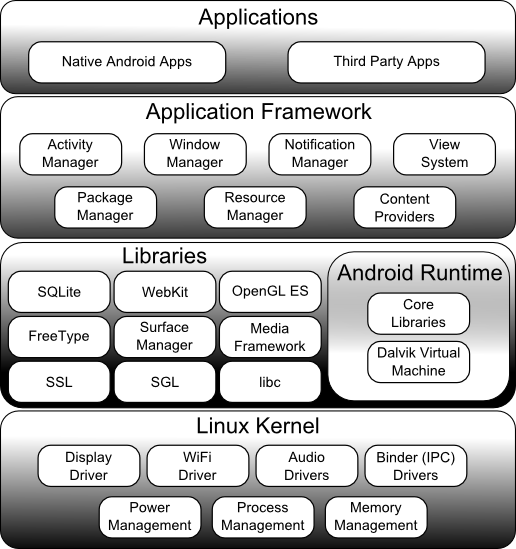
\includegraphics[scale=0.5]{figures/android_architecture.png}
 \end{center}
 \caption{Android architecture}
 \label{fig:android_architecture}
\end{figure}


\subsection{Linux kernel}

Android adopted a famous kernel with proven value concerning efficiency and security. Due to the wide set of constraints that mobile devices present comparing to desktop devices, the Linux kernel suffered some changes. It was properly modified in order to achieve exceptional results in an embedded environment. Therefore, the Android kernel is not a regular distribution of the Linux kernel, but a fork of the mainline kernel source code which allows the Android development team to both implement their necessary changes and follow the Linux kernel updates. This is a big advantage, because the Linux kernel is developed and maintained by a large community that releases, frequently, new patches and versions with enhancements, what lead Android kernel to adopt these enhancements. In fact, every new release of Android usually benefits from a new Linux kernel version. \autoref{tab:android_linux_versions} shows Android releases and the corresponding Linux kernel version.

\begin{table}
\begin{center}
\begin{tabular}{| l | l |}
\hline
\textbf{Android version} & \textbf{Linux kernel version} \\
\hline
Android Cupcake 1.5 & Linux kernel 2.6.27 \\
\hline
Android Donut 1.6 & Linux kernel 2.6.29\\
\hline
Android Éclair 2.0/2.1 & Linux kernel 2.6.29\\
\hline
Android Froyo 2.2 & Linux kernel 2.6.32\\
\hline
Android Gingerbread 2.3.x & Linux kernel 2.6.35\\
\hline
Android Honeycomb 3.x & Linux kernel 2.6.36\\
\hline
Android Ice Cream Sandwich 4.0.x & Linux kernel 3.0.1\\
\hline
Android Jelly Bean 4.1.x & Linux kernel 3.0.31\\
\hline
Android Jelly Bean 4.2.x & Linux kernel 3.4.0\\
\hline
\end{tabular}
\end{center}
\caption{Linux kernel versions and Android realeases}
\label{tab:android_linux_versions}
\end{table}

Google created the \gls{aosp}\footnote{http://source.android.com} to share the Android source code, that goes under the Apache Software License, Version 2.0, and related documentation. Since Android is a product of the Open Set Alliance, which includes a considerable amount of mobile manufactures that present different specifications of hardware, several branches of the Android kernel source code are kept on the git repository\footnote{https://android.googlesource.com}.

The way a mobile device operates is quite different from a laptop or desktop. As mentioned earlier, the Linux kernel suffered several modifications in order to fit a mobile device needs. It became an \textit{Androidized} kernel \cite{EmbeddedAndroid}. The following presents some of the most significant changes and new components brought to the kernel:

\begin{itemize}
 \item \textbf{Wakelocks} was one of the updated components. In Linux, the power management behaves according to the position of the lid in a laptop computer. If the lid is down, the power management will usually put the computer into "suspend" or "sleep" mode, the state of the processes is stored in RAM and the remain hardware turns off. This allows the laptop to save battery power. A mobile device should be in "sleep" mode as often as it is possible, but must not "sleep" when important processes are executing. Wakelocks are used to keep the system awake. Drivers developers need to grab and release wakelocks when important processing is being done or when an application is waiting for the user's input.

 \item \textbf{Low-Memory Killer} executes before the default kernel \gls{oom} killer. When the system lacks of free memory, processes can no longer allocate more memory and the kernel kills a task to get available space. This task is chosen based on priorities. Android's low-memory killer attributes \gls{oom} levels to processes depending on the components they are running and applies a threshold for each type of process. Android avoids the \gls{oom} state by reaching this threshold and killing tasks.

\item \textbf{Binder} is an \gls{ipc} mechanism adopted by Android that was based on OpenBinder. By \gls{ipc} we understand a framework that has the purpose of exchanging signals and data across multiple processes. It is used for message passing, synchronization, shared memory and remote procedure calls. Binder develops an important role among Android application components, as Content Providers, Services, etc \cite{Binder2013}.

\item \textbf{Anonymous Shared Memory (ashmem)} is another \gls{ipc} mechanism that is implemented as the POSIX SHM functionality, part of the System V IPC in Linux. However, the Android development team argued that this mechanism leads to resource leakage within the kernel \cite{EmbeddedAndroid}. Therefore, ashmem is based on POSIX SHM, but takes some enhancements. For instance, it uses reference counting to destroy memory regions when all processes have exited and reduces mapped regions when the system needs memory.

\item \textbf{Alarm} is another example of a driver that required some improvements comparing to the one of the default kernel. Android introduces the alarm timer, an hybrid solution that triggers a \gls{hrt} to fire when an event is supposed to run, while the system is running and, when the system suspends, the alarm timer looks at the list of events  and sets the \gls{rtc} to fire an alarm when the earliest event is to run \cite{AlarmTimer}.

\item \textbf{Logger} is a new mechanism of logging developed specially to Android. In Linux, typically, he find two logging systems: the kernel's own log, accessed through the \texttt{dmesg} command, and the system's log, stored at \texttt{/var/log/}. In Android there is a logger driver on the kernel that maintains circular buffers in RAM where it logs every incoming event \cite{Logger:eLinux}. This contrasts with Linux logging systems, because they use task-switches and file-writers to log each event, turning the process quite complex and heavy.

\end{itemize}

From a security point-of-view, Android inherited the user-based permission model from Linux that will be explained further. A new security feature was implemented on kernel, available as a build option called ANDROID\_PARANOID\_NETWORK, that restricts the access to some networking features, depending on the \gls{gid} of the calling process \cite{AndroidSecurity:AttackAndDefense}.


\subsection{Native Libraries}

Android has a considerable amount of dynamically loaded libraries that supports both Android system to execute internal tasks and  developers to use native code in their applications. Native libraries are written in C/C++, being available through the \gls{jni}. These libraries are placed at \texttt{/system/lib} in the Android filesystem. The following list presents the most relevant libraries:

\begin{itemize}
\item \textbf{Media Libraries} Enables playback and recording of audio and video formats. Based on OpenCore from PacketVideo;
\item \textbf{SQLite} Provides relational databases that can be used by applications and systems;
\item \textbf{SSL} Provides support for typical cryptographic functions;
\item \textbf{Bionic} System C library;
\item \textbf{WebKit} Browser-rendering engine used by Android browsers;
\item \textbf{Surface Manager} Provides support for the display system;
\item \textbf{SGL} Graphics engine used by Android for 2D.
\end{itemize}

\subsection{Android Runtime}

Android development team decided to use Java as the main language to build Android applications, because it is one of the most world wide used programming languages. In Java, there is a Java compiler that translate Java code into architecture-independent byte-code, which is executed at runtime by a byte-code interpreter known as "virtual machine". We are used to the \gls{jvm}. However, it is heavy to mobile devices. Therefore, Google decided to build a new "virtual machine" to deal with Java code and it is called \textit{Dalvik}. Apparently the name was stolen from a village in Iceland. The \gls{dvm} is designed to achieve good results in embedded environments, that uses slow CPUs, less RAM and are battery powered.


\subsection{Application Framework}

Similar to native libraries, the Application Framework offers a set of libraries to support developers. In this layer, libraries are written in Java and are available through Java APIs. The following list describes the most used libraries:

\begin{itemize}
\item \textbf{Activity Manager} Manages the activity lifecycle of applications and various application components. When an application requests to start an activity, Activity Manager provides this service;

\item \textbf{Resource Manager} Provides access to resources such as strings, graphics, and layout files;

\item \textbf{Location Manager} Provides support for location updates (e.g., GPS);

\item \textbf{Notification Manager} Applications interested in getting notified about certain events are provided this service through Notification Manager. For instance, if an application is interested in knowing when a new e-mail has been received, it will use the Notification Manager service;

\item \textbf{Package Manager} The Package Manager service, along with \textit{installd} (package management daemon), is responsible for installing applications on the system and maintaining information about installed applications and their components;

\item \textbf{Content Providers} Enables applications to access data from other applications or share its own data with them;

\item \textbf{Views} Provides a rich set of views that an application can use to display information.

\end{itemize}



\subsection{Applications}

The top layer is composed of the main pieces of the entire system: applications. Android usually comes with several applications, as browser, mail, contacts, etc. Through Google Play, and other third party markets, users may download and install applications that are no different from those previously installed on the device. Android applications present the following filesystem structure:

\begin{itemize}
\item \texttt{src} includes the java packages and files;
\item \texttt{gen} holds auto generated code for resources;
\item \texttt{Android x} contains the android jar file for the targeted version of Android, denoted by \texttt{x} (for instance, \texttt{Android 2.3.3});
\item \texttt{assets} comprises those files that the developer bundles to the application;
\item \texttt{bin} stores files for compiling and running the application, as the \textit{apk} file and \textit{classes.dex} files;
\item \texttt{res} contains all application resources: layouts, values (like strings) and drawables;
\item \texttt{AndroidManifest.xml} defines the application components;
\item \texttt{proguard-project.txt} is the proguard configuration file.
\end{itemize}

Later in this document several references to Android folders will be made.

\section{Android Components}

The following sections present the Android components by which applications consists of. Each component was designed to develop a special role in the application's life and some rules need to be carried out in order to get the desired behavior as well as efficiency. 

\subsection{Activities}

Android provides the application's visual interface through the \textit{Activity} component. Once created, it exhibits elements that users can interact with, like buttons, text boxes, spinners, etc. When developers are implementing Android activities, concepts regarding visual design must be taken into account so that users may have a pleasant experience. Regular applications have several activities, because the visual interface changes according to the user's desire, while he keeps tapping and clicking along the application's execution. Android provides mechanisms to save activities state when they are paused or stopped and keeps them in a stack so that they can be restarted later. This process is presented in \autoref{fig:act_lifecycle} that illustrates the activity lifecycle\footnote{http://developer.android.com/guide/components/activities.html}.

\begin{figure}[h]
 \begin{center}
 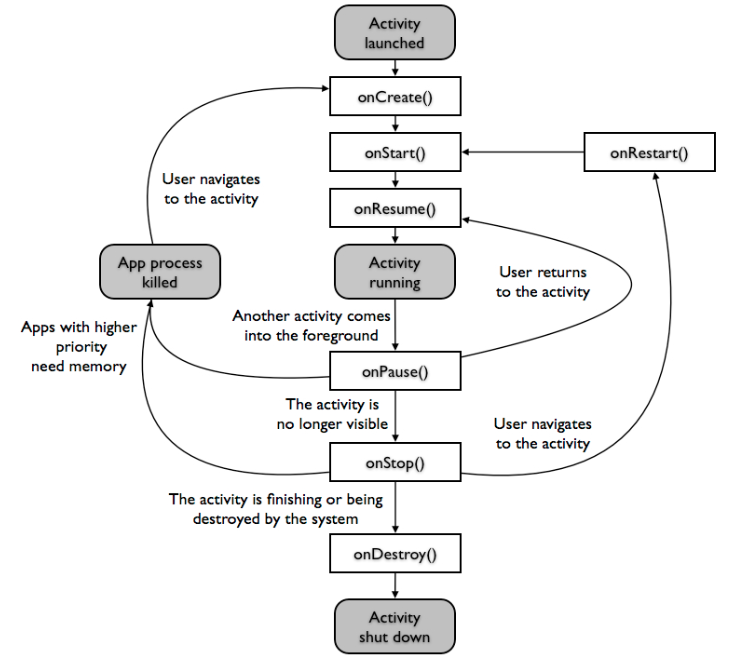
\includegraphics[scale=0.5]{figures/activity_lifecycle.png}
 \end{center}
 \caption{Activity lifecycle}
 \label{fig:act_lifecycle}
\end{figure}

Activities begin the execution calling \texttt{onCreate()} that, usually, defines the layout for the activity's user interface. The activity becomes visible when \texttt{onStart()} runs. Once the activity is visible, \texttt{onResume()} takes place and the activity just stops being visible when another activity comes to the foreground. When this happens, \texttt{onPause()} is called. If the system needs memory to execute activities with higher priority, the activity is killed. If the activity is requested to run again, it can continue the previous task. The activity may also be stopped through \texttt{onStop()}. While stopped it cannot go back to the previous task, but might be restarted through \texttt{onRestart()}. At last, the activity is destroyed calling \texttt{onDestroy()}. The activity's lifecycle ends.

\subsection{Services}

When developers intend to launch some task that has no visible elements they use \textit{Services}. This component is designed to perform long running operations in the background. For this reason, a service is able to run even if the component that called it, or even the application, stops its execution. Services usually take care of operations like internet downloads, music playing, etc.

\begin{figure}[h]
 \begin{center}
 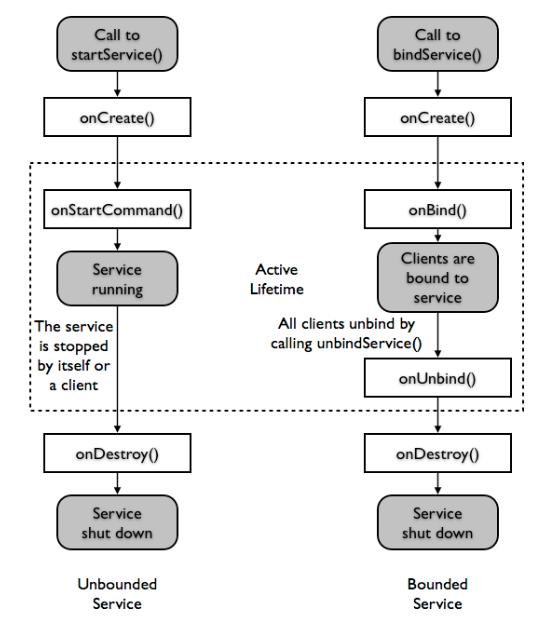
\includegraphics[scale=0.5]{figures/service_lifecycle.png}
 \end{center}
 \caption{Service lifecycle}
 \label{fig:serv_lifecycle}
\end{figure}

Services may be called in two distinct ways. An application component, as an activity, may start a service calling \texttt{startService()}. It may run in the background  indefinitely, even if the component that started it is destroyed. After completes its operations, the service should stop itself.

In the other way, a service can be bound to an application component, if this binds to it by calling \texttt{bindService()}. In this case, the service executes using a service-client interface providing interaction with components, as sending requests, getting results, etc. A bound service runs while it is bound to some application component, being destroyed after that. Note that the same service may assume both forms, unbound and bound.

The service lifecycle shows these two approaches in \autoref{fig:serv_lifecycle} \footnote{http://developer.android.com/guide/components/services.html}. On the left side we can see that an unbounded service starts its work by calling \texttt{onStartCommand()}. After performing it may be stopped by a client or by itself, calling \texttt{onDestroy()}. In a bounded service, \texttt{onBind()} starts its execution and when all clients unbind the service, it calls \texttt{onUnbind()} and \texttt{onDestroy()}.

Services play a major role in the scope of this project, because it's through a service that Droidguardian is able to perform indefinitely in the background, being started when the device boots, as we will explain further.

\subsection{Broadcast Receivers}

Broadcast receivers are built to handle events created by applications or by the system. Receivers are designed to perform a certain action when notified that some event occurred. For instance, a receiver can be set to start an activity when the device boots. The developer registers the action \texttt{BOOT\_COMPLETED} wrapped in a package called \textit{intent}. When the system performs this action, sends the package to the receiver. The receiver checks the action inside. If it is the desired action, the receiver sends another package to the system requesting an activity to start. Receivers must always be associated with intents. An \textit{Intent} is a messaging object that connects all components in an Android applications by allowing them to be invoked and sharing some data\footnote{http://developer.android.com/guide/components/intents-filters.html}. \autoref{fig:broadcast_rec} exhibits the way application components use intents to communicate.

\begin{figure}[h]
 \begin{center}
 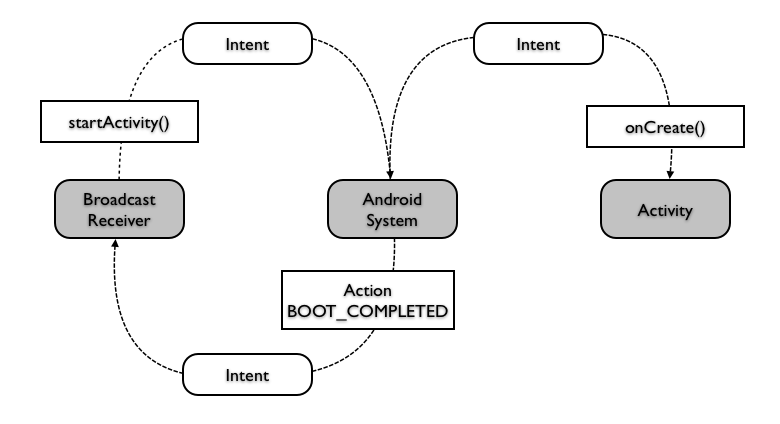
\includegraphics[scale=0.5]{figures/broadcast_receiver.png}
 \end{center}
 \caption{Broadcasting an intent to start an Activity}
 \label{fig:broadcast_rec}
\end{figure}


\subsection{Content Providers}

It is common that Android applications need to access and share some resources in order to provide the user useful features. These resources can be user's personal data, as videos, audio, images, contacts, etc. Android supplies a consistent standard interface to data that also handles \gls{ipc} and secure data access. \textit{Content providers} offer this mechanism as an application component, by which it allows the application to access a data repository. Providers are primarily designed to be used by other applications, even though they can be called only to manage its application's internal data. Providers present data to external applications using a relational database like interface, providing CRUD (create, retrieve, update and delete) functions and a \gls{uri} system\footnote{http://developer.android.com/guide/topics/providers/content-providers.html}.

\chapter{Android Security}
\label{chap:android_security}
Android was designed to protect applications considering both security-oriented developers and those less familiar with safety concerns. By default, Android enforces good levels of protection, inheriting the Linux security model, but also applying its own mechanisms. It is provided with a multi-layered security that supplies the flexibility required for an open platform, while providing protection for all users of the platform\footnote{http://source.android.com/devices/tech/security}. This chapter introduces a general overview into Android security features.

\section{System and Kernel Level Security}

The Android platform comprises three main blocks: device hardware, operating system and application runtime. Each block presents secure mechanisms that are briefly described in the following sections. 

\subsection{Linux Security}

Android has inherited security mechanisms from the Linux kernel, namely, a user-based permissions model, process isolation and extensible mechanism for secure \gls{ipc}. The user-based permissions model was originally developed for Unix environments, thus Linux takes advantage of it. In fact, the user-based permissions model has proven its good design concerning security issues over time. Every user registered in the system has an unique identifier number known as \gls{uid}. Along with users, there are groups that are identified by its unique \gls{gid}. One group might have one or more users, and one user might belong to one or more groups. Note that all users belong to at least one group, which is the group that contains all users. Every resource in the system, or in simple terms, every file in the system has an owner, that is identified by its \gls{uid}. This owner has the responsibility over the file and is able to alter its permissions. Files have also a group associated which is identified by its \gls{gid}. Each file on a Linux system has three sets of permissions: owner, group and world. The owner and the group are those mentioned before. The world is considered to be every user registered on the system. Each file might be accessed by three types: read, write and execute. So, each set of permissions can include read (r), which allows an entity to read the file; write (w) which allows an entity to write the file; and execute (x) which allows an entity to execute the file. According to its permissions, a file may be read and/or wrote and/or executed by its owner, that has an unique \gls{uid}, and/or by every member of the file's group, and/or by all other users that have an account on the system \cite{ComputerSecurity}.

\subsection{Application Sandbox}

Using the user-based permissions model, the system's resources have a robust access control. Android took this feature and built an application sandbox where each application can only access its own files and components (unless the developer grants other permissions that we'll see later). When an application is installed on the system, an new unique \gls{uid} is assigned to it and the application runs under this \gls{uid}. In addiction, all data stored by that application is assigned the same \gls{uid}. The Linux permissions are set on this application to allow read, write and execute access by its owner and no permissions otherwise. This mechanism is illustrated in \autoref{fig:android_sandboxing} \cite{AndroidSecurityUnderpinnings}.

\begin{figure}[h]
 \begin{center}
 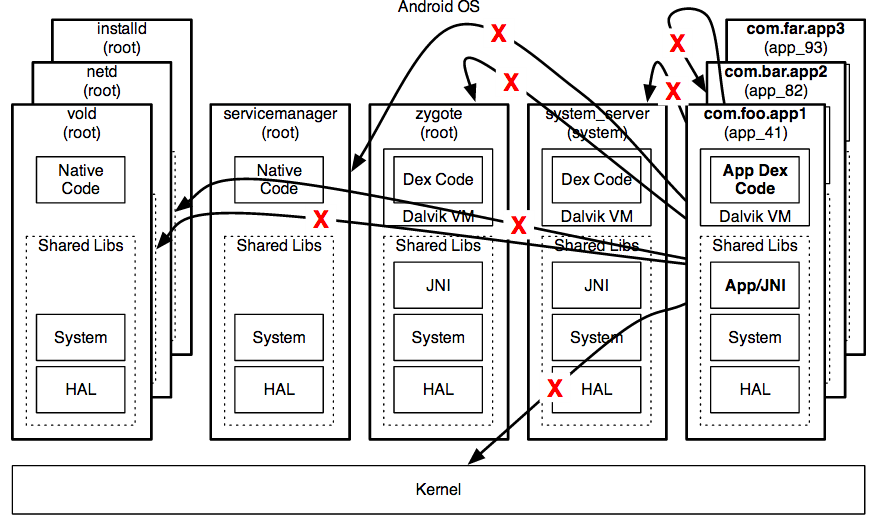
\includegraphics[scale=0.5]{figures/android_security.png}
 \end{center}
 \caption{Application sandboxing}
 \label{fig:android_sandboxing}
\end{figure}

\subsection{Filesystem Isolation}

The user-based permissions model is also used to provide filesystem isolation, which fits in the application sandboxing model. Android creates a specific directory to each installed application under the path \texttt{/data/data/}. Each directory is configured such that the associated application's \gls{uid} is the owner and only its permissions are set. Within this directory is \texttt{/files} directory that stores all files created by the application. These files are granted the same permissions and run under the owner's \gls{uid}, providing isolation access from other applications. This access control is enforced to all applications. However, if a user access the Linux kernel using the root \gls{uid} will break down the sandboxing mechanism and be able to access any data stored in any application.

Linux permissions access control works on every Android filesystem except on the SD card (\texttt{/sdcard} directory). Therefore, any file written to external storage is accessible by any application.

\subsection{Security-Enhanced Android}

As mentioned above, the user-based permissions model grants protection from the Android foundations. However this model enforces a \gls{dac} mechanism that increases the risk of harm, as we will see later in the \gls{lsm} section. To overcome the related threats, Android began to use a component that has been in the Linux kernel in the last years, \gls{sel}. This mechanism applies a \gls{mac} model \cite{SEAndroid} that reduces the effect of malicious software and protect users from potential flaws in code\footnote{http://source. android.com/devices/techsecurity/se-linux.html}. 

\section{Android Application Security}

Android applications extend the core Android operating system. The previous security features were not able to ensure the protection level desired to a world wide used mobile platform as Android, therefore a set of artifacts were developed granting applications safety in a satisfactory degree. They are briefly described as follows.

\subsection{Manifest Permissions}

Besides the user-based permissions model adopted from the Linux kernel, Android brought a new permissions model know as \textit{Manifest permissions}. As mentioned earlier, each application is only allowed to access its own data, by default. However, Android offers a lot of resources and libraries so that developers can build powerful and useful applications. But, the gain of power brings security vulnerabilities. For instance, Android provides network resources that allow applications to establish internet communications. But, malicious applications could take advantage of this feature and use it to spread user's personal data.


Google decided to implement the Manifest permissions model that forces developers to specify which resources their applications use when executing. Each resource requires a permission that must be declared on the Manifest file. At installation time, permissions are set to the application and it will only have access to the declared resources. Using the previous example, if the developer wants to use network resources, he declares the INTERNET permission through the following statement:

\noindent \texttt{<uses-permission android:name="android.permission.INTERNET"/>}

\noindent on the Manifest file. Before the installation, the user gets the list of all Manifest permissions. This feature brings two main advantages. First, it alerts the user to all possible dangerous actions the application may take. For instance, if the user intends to install a simple game and the Manifest file exhibits SMS and phone call permissions, which means that the application can send SMS and make phone calls, something doesn't seem to be right. The user makes his judgement and decides to either install or not install the application. The second advantage ensures the protection of the application against malware. In the case of one application gets compromised, the attacker will only be able to access the resources that the application was allowed to. For instance, if an application that takes photos has only permission to use the camera and gets compromised, the attacker will only be able to access the camera and none of the remaining resources that need Manifest permission.


Android comprises a large set of Manifest permissions\footnote{http://developer.android.com/ reference/android/Manifest.permission.htm} and regular applications take advantage of a considerable amount of them. Since there is a considerable set of permissions that causes no harm to the device, users don't need explicitly to accept them in order to install applications. Therefore, Google established four categories where Manifest permissions falls into, described as follows:

\begin{itemize}
 \item \textbf{Normal}. Permissions to access inoffensive resource. For that reason they are granted by default. As example, the permission to change the device's background;

 \item \textbf{Dangerous} Permissions to access resources that might cause harm to users. In this case, users must accept them before the installation. As example, the permission to access 
private data, or establish internet connections;

\item \textbf{Signature} Permissions that were required by other applications signed with the same digital certificate. If the application is signed by the same certificate as the declaring app, the permission will be granted; if not, the app being installed will no be granted the permission. The user is never questioned about these permissions in order to start an installation;

\item \textbf{SignatureOrSystem} These permissions follows the same rule as \textit{Signature} permissions, but adding a new rule that checks the Android system image. This type of permission is used by device manufacturers to allow applications created by different vendors to work together within that Android builds.
\end{itemize}


An important rule that follows the Manifest permission is the Principle of Least Privilege \cite{ApplicationSecurity:Oreilly}, which states that each application should keep permissions at its minimum, using the weak permission instead of a strong one that allows the application to execute tasks that will not be called. For instance, if the application only needs to read contacts, the permission required should be \texttt{READ\_CONTACTS} and not full access to contacts that also allow to write contacts.

\subsection{Application Signing}

Google requires all Android applications to be signed through a digital certificate, being the private key held by the application's developer. This process ensures the authentication of a developer when he's trying to deploy his application into the market and establishes trust relationships between applications. Signing an application does not require a \gls{ca}. In fact, most of Android applications are self-signed by developers. Google released tools that allow developers to sign their applications and provides useful documentation to facilitate the process\footnote{http://developer.android.com/tools/publishing/app-signing.html}.


The Application signing process concede an useful feature to developers that build more than one application. As mentioned earlier, each application is assigned an unique \gls{uid} and is not allowed, by default, to share data and resources with other applications. However, if an user installs more than one application signed by the same developer, which means the same digital certificate, and these applications declare the \texttt{shareUserId} attribute in the Manifest file, Android assigns these applications the same \gls{uid}. Therefore, they are seen by the Linux kernel as the same application and are able to share data and resources.

\subsection{Android Security Overview by Google}

Android Security chief, Adrian Ludwing, presented the Google's approach to fight malware and statistical data regarding infected devices \cite{VBAndroidPracticalSecurity} . Android enforces several layers of protection since the user accesses Google Play until the application is running on its device. These layers were introduced as follows:

\begin{itemize}
\item Google Play;
\item Unknown Sources Warning;
\item Install Confirmation;
\item Verify Apps Consent;
\item Verify Apps Warning;
\item Runtime Security Checks;
\item Sandbox and Permissions.
\end{itemize}

Google Play requires developer information and application signing. Furthermore, each application is reviewed before it becomes available. This process involves a set of procedures that checks static code dynamic behaviors. Heuristics and similarities on-device data are applied. After the analysis it is assigned a probability of threat tag to the application, being \textit{Block}, \textit{Warn} or \textit{Allow}.

Android does not allow the installation of applications from unknown sources by default. This feature ensures that all installed applications had passed the Play Store test. If the user disables this rule by allowing unknown sources, the following alert is displayed \textit{"Your phone and personal data are more vulnerable to attack by apps from unkown sources. You agree that your are solely responsible for any damage to your phone or loss of data that may result from using these apps"}. Also, the feature \textit{Verify Apps} inspects applications prior to install, applying an additional layer of security. If the application presents suspicious code, the installation process might be blocked, in sever cases, or triggers a warning. This is quite useful for those applications that skip the Google Play process review, i.e. were installed from third-party sources.


\chapter{Related work}
\label{chap:background}
% Background

Droidguardian was inspired by a powerful tool called \textit{Little Snitch}, that aims to raise awareness regarding internet connection attempts from the system's applications. Little Snitch provides a graphical interface so that users can filter outgoing internet connections\footnote{Later versions of Little Snitch allow to manage incoming internet connections as well, but this feature is out of this project scope.} through rules and accept or reject connections in real time. In order to develop Droidguardian, a deep study and understanding of Little Snitch took place and the following section will cover the relevant details. It might be important to stress the fact that Little Snitch is designed exclusively for Mac OS X operating system and it is not open source. All information presented below stems from both the use of the tool and available documentation reading.

Since Android is an embedded Linux environment product, in the initial research phase to design Droidguardian we stumbled upon a very interesting tool, quite similar to Little Snitch, although much simpler, called \textit{TuxGuardian}. This tool aims to exhibit in real time all outgoing internet connection attempts, allowing users to accept or reject such connections. TuxGuardian was designed for Linux based operating systems and is open source, which led to a thorough analysis introduced later in this chapter.

\section{Little Snitch}
\label{sec:little_snitch}

Little Snitch\footnote{http://www.obdev.at/products/littlesnitch/index.html} is by definition a firewall built for Mac OS X. However, it is not a regular firewall that operates at network packet level, checking protocol headers, but a firewall that acts at higher level, closer to the application layer. Little Snitch is set to intercept network connections attempts originated from all the system's applications and processes. Once a network connection attempt occurs in the system's kernel, it is intercepted by Little Snitch which will either accept it or reject it. This decision is based on a set of rules created by the user and by Little Snitch. The following section introduces Little Snitch rules.

\subsection{Little Snitch rules}

A rule is composed of four elements:

\begin{itemize}
\item Condition
\item Action
\item Lifetime
\item Annotations
\end{itemize}

When an application, or Unix process, tries to establish an internet connection, it passes to the system some required data, as an address and a port. These data is collected by Little Snitch that compares it to the existing rule. The \textit{condition} field of each rule has the following properties:

\begin{itemize}
 \item Process
 \item Process owner
 \item Server
 \item Port
 \item Protocol
 \item Direction
 \item Enabled
\end{itemize}

An internet connection might be seen as a triplet that includes a server, a port and a protocol. It has associated the process that triggered the connection and the owner of the process. The server is the remote internet address and Little Snitch handles them using numeric sets, \gls{dns} hostnames and \gls{dns} domains. The port points to services. Protocols (\gls{tcp}, \gls{udp} or \gls{icmp}) states the behavior of the internet connection. Processes are applications, as Safari, Mail, etc, and UNIX processes, as \textit{storeagent}, \textit{ntpd}, etc. These processes are owned by an entity, as System, root, etc. There are two other properties that belongs to conditions: connection direction and enabled. The first one indicates if the connection is incoming or outgoing and the last one may be seen as a flag that states if the rule is on or off.

Connection attempts are compared to these properties and, if a match occurs, the matched rule takes its action. A connection that matches an off enabled rule is not handled. The action is one of the following:

\begin{itemize}
 \item Allow
 \item Deny
 \item Ask
\end{itemize}

It's easy to understand that the rule may either allow or deny the connection. In the first case, the connection is established as if it was not intercepted by Little Snitch. In the second, the process attempting the connection receives an error, like a network failure, and the connection does not take place. The ask action is triggered when Little Snitch does not have the connection data stored, in a sequence of either being the first time the connection occurs or the user didn't want to save it earlier. Therefore, Little Snitch launches a dialog message, called \textit{Connection Alert}, reporting the connection attempt, revealing the connection properties and providing choice buttons so that the user may decide what to do. \autoref{fig:ls_dialog} shows a Little Snitch Connection Alert window. The figure reveals the Connection Summary, a short text indicating the server (\textit{ax.init.itunes.apple.com}), the port (\textit{80}) and the protocol (\textit{http}); the Action, composed by the choice buttons \textit{Allow} and \textit{Deny}; the Rule Lifetime, where the user assigns a time tag to the rule; Rule Options to determine if this application (\textit{iTunes}) is allowed to established every connection or if there are some restrictions regarding the server, port and protocol. At last, the Research Assist Button exhibits some detailed information about the connection's properties that may help users to decide what to do.

\begin{figure}[h]
 \begin{center}
 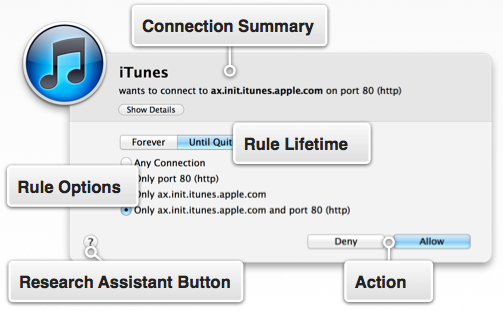
\includegraphics[scale=0.5]{figures/LS_Dialog.png}
 \end{center}
 \caption{Little Snitch Connection Alert window}
 \label{fig:ls_dialog}
\end{figure}

Rule Lifetime plays an important role. It allow users to define the frequency they want that connection to occur. He can choose one of the following tags:

\begin{itemize}
\item \textit{Forever} - The rule never expires;
\item \textit{Until Quit} - The rule expires when the last instance of the process that matches the rule terminates;
\item \textit{Until Logout} - The rule expires when the user who created the rule logs out;
\item \textit{Until Restart} - The rule expires when the computer is restarted;
\item \textit{Minutes} - The rule expires a certain amount of time after it was created;
\item \textit{Once} - The connection takes places and the rule is not saved.
\end{itemize}

The descriptions above explain how Little Snitch perform. For instance, a \textit{forever} rule will only display a Connection Alert once. All matching connections after the rule is setted up will be executed according to the action's rule. On the other side, if the user chooses the \textit{once} tag, is either allowing or denying the connection only this time and desires to be notified if it happen again. In this case, the Connection Alert will be prompt as if it was the first time this connection appears in the system.

As mentioned earlier, Little Snitch is a powerful tool. It has a mechanism to distinguish important processes that need to establish internet connections in order to keep the system executing without problems. These processes are automatically granted permission to connect to external servers. However, the user may check the related rules and change them. For this reason, Little Snitch provides the \textit{Annotation} field, in which rules are characterized as \textit{Protected} or \textit{Unapproved} to inform the user about their special status. Besides this feature, Little Snitch provides different profiles to each network the system is connected, and other useful features that make this tool quite robust and valuable.

\subsection{Little Snitch architecture}

A simple version of Little Snitch architecture is presented in \autoref{fig:ls_architecture}. At the bottom we find a Kernel Extension responsible for the interception of connection attempts. The ability to refuse an internet connection cannot be performed at user level. Therefore, Little Snitch developers was forced to operate at kernel level, building a Kernel Extension \cite{Documentation:LittleSnitch}. The collected data from the bottom layer is sent to the layer above, the Network Filter. The matching process is done in this layer. At the top is placed the user interface that permit users to check information, define rules, etc.

\begin{figure}[htbp]
 \centering
 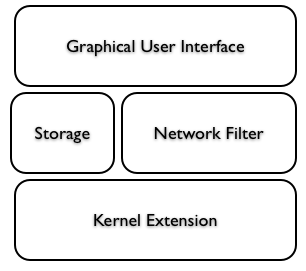
\includegraphics[scale=0.5]{figures/ls_arch.png}
 \caption{Little Snitch architecture}
 \label{fig:ls_architecture}
\end{figure}


% TuxGuardian

\section{TuxGuardian}
\label{sec:tuxguardian}

TuxGuardian\footnote{ http://tuxguardian.sourceforge.net} is an open source tool designed for Linux based operating systems, that intercepts outgoing internet requests and triggers notification alerts to the user. Its basic behavior is quite similar to Little Snitch. Although this tool stopped being updated since 2006, it was very important in the scope of this project and played a major role in Droidguardian's development process. In fact, that's where the name \textit{Droidguardian} came from. The following sections presents TuxGuardian in detail.

\subsection{TuxGuardian architecture}

TuxGuardian is a host firewall that emerged to overcome the complexity of Linux security model to lay users, providing an interface to implement access control policies to the network outgoing traffic. It consists of a three layered architecture showed in \autoref{fig:tg_architecture}. Each layer has a specific function and establishes a communication to the next layer. 

\begin{figure}[htbp]
 \centering
 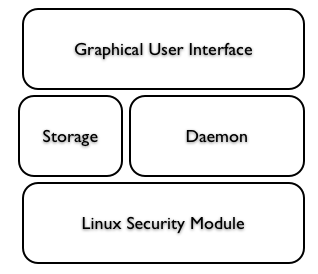
\includegraphics[scale=0.5]{figures/tg_arch.png}
 \caption{TuxGuardian architecture}
 \label{fig:tg_architecture}
\end{figure}

The \textit{Security Module} is the bottom layer and takes advantage of the \gls{lsm} framework  to implement hook functions that grab internet socket requests. Namely, TuxGuardian uses the callback functions \texttt{socket\_create} and \texttt{socket\_listen} to intercept both socket client and socket server internet connection requests\footnote{For the sake of simplicity, we will not cover security modules framework in this chapter, but it will be detailed later in this document.}. Local socket requests are not handled. Through this mechanism, TuxGuardian is able to block outgoing connections. In the same way as Little Snitch, this operation must be executed in kernel space. When the security module detects a connection attempt, sends a message to the layer above and waits a response in order to either deny or allow the connection.

The \textit{Daemon} is by definition a program that executes in background waiting for some event to take place. In this case, it waits for the security module messages, that consists of the \gls{pid} of the process that created the connection request. This communication process is established through local sockets. When the daemon gets the security module's message, checks the storage file to find a connection match. This procedure is also very similar to Little Snitch. If a match is found, TuxGuardian executes the corresponding action. Otherwise, it launches a notification window to get the user's response. Note that TuxGuardian is able to perform without the \gls{gui} component, denying all connections that are not placed in the storage file. In order to enforce a security measure, TuxGuardian keeps the MD5 hash of each process path. Through \gls{pid}s, the daemon gets the process path name in the \texttt{/proc} directory and calculates its MD5 hash so that modified programs cannot access internet.

The \gls{gui} or \textit{Frontend} displays the notification windows. The user receives the process name (the complete process path, for instance \texttt{/bin/ping}) that created the connection attempt and decides to either accept it or reject it. Along with the process path, the corresponding MD5 hash is also displayed. \autoref{fig:tg_dialog} presents the TuxGuardian notification window.

\begin{figure}[h]
 \begin{center}
 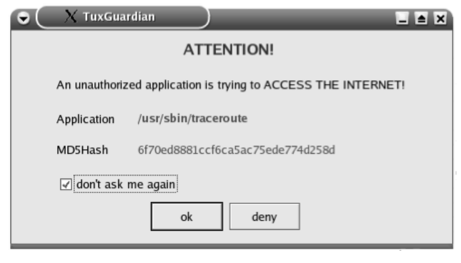
\includegraphics[scale=0.5]{figures/tg_dialog.png}
 \end{center}
 \caption{TuxGuardian notification window}
 \label{fig:tg_dialog}
\end{figure}

\subsection{TuxGuardian Protocol}

The communication between layers is established through the \gls{tgp} \cite{Report:TuxGuardian}. This comprises a structure with the following fields:

\begin{itemize}
\item Sender
\item Sequence number
\item Query type
\item Query data
\end{itemize}

\textit{Sender} specifies the layer which sent the message: 

\begin{itemize}
\item \texttt{TG\_MODULE},
\item \texttt{TG\_DAEMON},
\item  \texttt{TG\_FRONTEND}
\end{itemize}

corresponding to the security module, the daemon and the frontend, respectively. \textit{Sequence number} acts as the message identifier. \textit{Query type} characterizes the message, or query, as follows:

\begin{itemize}
\item \texttt{TG\_ASK\_PERMIT\_APP} refers to the query sent by the security module to the daemon asking permission to either allow or deny the connection request;
\item \texttt{TG\_RESPOND\_PERMIT\_APP} refers to the response the security module gets from the daemon to the question above. \textit{Query data} field stores the permission value;
\item \texttt{TG\_PERMIT\_SERVER} refers to the first query, but indicating that the connection request involves a server;
\item \texttt{TG\_RESPOND\_PERMIT\_SERVER} refers to the response obtained from the previous question.
\end{itemize}

Depending on the nature of the query, \textit{Query data} may store a \gls{pid} or the permission values: either \textit{yes} or \textit{no}. 

\section{Related Android Apps}


Several mechanisms have been implemented to enforce fine-grained access policies regarding network connections on Android devices. \textit{Aurasium} provides a security feature that isolates each application in a custom sandbox controlling the access to the device's data and resources. It defines a set of rules and policies that ensure the device's protection. Aurasium provides a technology that repackages each \texttt{apk} file applying an intermediate layer that intercepts certain operation calls that use value resources, as Internet, SMS messages, IMEI, contact information, etc. Each access is conditioned by a set of policies which may be defined automatically or by the user. 

One of the most interesting features of this tool is the ability to enforce its policies without modifying the Android system. Aurasium places native code in the native framework layer and through 

 what makes it easily and widely deployed. Regarding network access, Aurasium authors state that independently from the level a network operation is called, it will fall on the \texttt{connect()} method in the \texttt{OSNetworkSystem} Java class. This method calls the \texttt{libnativehelper.so} library that transfers control to the \texttt{connect()} method of the \texttt{libc.so} library. At last, the socket is able to get connected by libc delivering a system call to the Linux kernel. This path allows to create a check point above the Linux kernel in order to monitoring all operations called by the uppermost layers. By controlling the Bionic libc library, Aurasium is able to execute a set of policies that protect the entire Android system \cite{Aurasium}.


Malicious applications take advantage of the Manifest permissions to grant access to resources that the user is not aware of when installing such apps. Even though these permissions are presented before the installation process, the user is not able to figure out if is granting permission to his valuable assets. In order to apply a control level between Manifest permissions and those permissions Android apps really need, it was developed an interesting mechanism called \textit{AppFence}. This tool inspects the app's Manifest permissions and allows users to decide which should be applied and those that should not, overtaking the obligation of accepting all permissions in order to install the app. In fact, all permissions are accepted, but instead of granting access to certain resources, AppFence replaces them with \textit{shadow data}, which is an inoffensive imitation of that resources. For instance, if an app requires access to the contacts list and the user do not agree, the system will provide an empty list to the app. If the application is bad intentioned regarding that list, it will cause no harm to the user.
AppFence also protects against data leakage through outgoing connections. It performs at socket level by intercepting data buffers. When the malicious app is writing to a buffer, AppFence acts in one of two ways: tricks the app by indicating that the buffer was been sent or emulates a state in which the device has no wireless connections.


presents an interesting work regarding network policies where the author states that Android's internet static permission provides a coarse grained permission. He claims that 






\chapter{Technical concepts}
\label{chap:technical_concepts}
The development process of DroidGuardian required some technical concepts. This chapter introduces these concepts along with relevant details to the scope of this project.

\section{Loadable Kernel Modules}
In Linux systems it is possible to develop kernel routines and run them as if they were part of the kernel. This is accomplished through \gls{lkm} which are programs written specifically to the kernel that can be loaded at runtime. This feature brings a lot of advantages to developers enabling them to access low level resources from the kernel. Simple modules are easily written and installed. However, they are usually built to perform complex tasks at kernel level, leading to complex source code. When playing with kernel modules, developers must ensure that the code is not corrupted in any way, otherwise the system may stop abruptly leading to an unrecoverable state (usually designated as kernel panic).

\subsection{Building}

In order to get a \gls{lkm} to run on the kernel, the user must provide the \textit{entry} and \textit{exit} points. The former is called when the module is inserted into the kernel. The last is called when the module is removed from the kernel. 

The entry point is implemented as a function that is declared as \texttt{static} and should return the \texttt{int} value of 0. This \textit{init} function may have any name, and is defined as the entry point through the \texttt{module\_init()} primitive. For instance, if the init function is called \textit{"hello"}, the entry point is defined as follows:

\begin{lstlisting}[caption=Defining the Loadable Kernel Module's entry point]
module_init(hello);
\end{lstlisting}

The exit point is implemented as a function that is also declared as \texttt{static} but returns \texttt{void}. Similar to the entry point, the exit function may assume any name, but this should be passed as argument to the \texttt{module\_exit()} primitive. For instance, naming the exit function as \textit{"goodbye"}, the exit point is defined as follows:

\begin{lstlisting}[caption=Defining the Loadable Kernel Module's exit point]
module_exit(goodbye);
\end{lstlisting}

\subsection{Compiling}

The compilation process is accomplished using the \textit{make} utility. The developer should build a \textit{Makefile} providing the path to both the module's location and the kernel's libraries that will generate the \texttt{.ko} file. A simple example of such \textit{Makefile} is presented as follows:

\begin{lstlisting}[caption=Example of a Makefile to compile Loadable Kernel Modules]
obj-m := example_module.o

KDIR := /lib/modules/$(shell uname -r)/build
PWD := $(shell pwd)

all:
        $(MAKE) -C $(KDIR) M=$(PWD) modules

clean:
        $(MAKE) -C $(KDIR) M=$(PWD) clean
\end{lstlisting}

The source code file of the module above is called \texttt{example\_module.c} and the originated module file will be called \texttt{example\_module.ko}. Note the \texttt{uname -r} command that will give the kernel's version so that the compiled module is able to run in the same kernel. Developers must pay attention to kernel's versions in order to build compatible modules.

\subsection{Inserting and Removing}

Linux provides several commands to deal with kernel modules. To insert modules into the kernel, developers use the \texttt{insmod} command that takes a \texttt{.ko} file as argument. For instance, to insert the module presented above, the following command is executed:

\begin{lstlisting}[caption=Linux command to insert Loadable Kernel Modules]
# sudo insmod example_module
\end{lstlisting}

After executing this command, the module starts to run immediately by calling the entry point function. To remove the module, the following command must be executed:

\begin{lstlisting}[caption=Linux command to remove Loadable Kernel Modules]
# sudo rmmod example_module
\end{lstlisting}

\section{Interprocess Communication using Sockets}
\label{sec:sockets}
Unix provides several solutions to perform \gls{ipc}. Sockets use file descriptors to fulfill this task. This section introduces relevant details regarding both internet sockets and local (Unix domain) sockets focusing on the stream socket type. Also, sockets are handled differently regarding the virtual memory of the system: user space and kernel space. Firstly we'll present a simple server-client model implementation at user space followed by some particularities of socket implementation at kernel level.

\subsection{Stream Sockets}

Unix systems provide a programming interface to easily carry out \gls{ipc} tasks using sockets. This \gls{api} is present in the \texttt{sys/socket.h} header file. Sockets follow a server-client based model, in which a sequence of primitives needs to be invoked in order to established the connection. This sequence depends on the protocol that will take place. Usually, sockets fall into the \gls{tcp} or \gls{udp} protocols. Both require different primitives to settle connections. In the scope of this project, only stream sockets are used. Therefore, this section will focus on the basic behavior of stream sockets. \autoref{fig:server_client_sockets} illustrates a typical case and may be described as follows:

\begin{figure}[h]
 \centering
 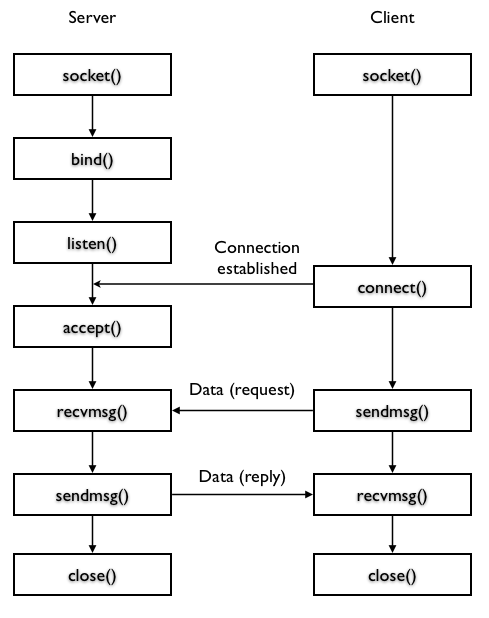
\includegraphics[scale=0.5]{figures/server_client_sockets.png}
 \caption{Typical server-client based model of stream sockets}
 \label{fig:server_client_sockets}
\end{figure}

\begin{enumerate}
\item The server initializes the process by creating a file descriptor (socket descriptor). This process is accomplished through the \texttt{socket()} primitive:

\begin{lstlisting}[caption=Declaration of the \texttt{socket()} function]
int socket(int domain, int type, int protocol);
\end{lstlisting}

The returned value defines the socket descriptor. As arguments, \textit{domain} specifies the socket family (\texttt{AF\_INET}, \texttt{AF\_INET6}, \texttt{AF\_UNIX}, etc), \textit{type} specifies the socket type (\texttt{SOCK\_DGRAM}, \texttt{SOCK\_STREAM}, etc) and \textit{protocol} indicates a particular protocol to be used with the socket, but usually takes the value 0.

\item Once created, the socket is unnamed and needs to be bound to an address in order to be identified by the system. This address will be assigned depending on the socket family. The \texttt{bind()} primitive is presented as follows:

\begin{lstlisting}[caption=Declaration of the \texttt{bind()} function]
int bind(int socket, const struct sockaddr *address, socklen_t address_len);
\end{lstlisting}

If the returned value is 0, the operation was successful. In case of error, returns -1. The argument \textit{socket} specifies the socket descriptor previously created, the \textit{address} points to the address to be bound to the socket and \textit{address\_len} indicates the length of the address structure.

\item After the binding, the server is ready to establish a connection to a client. Thus, the server is kept listening to connection requests through \texttt{listen()}:

\begin{lstlisting}[caption= Declaration of the \texttt{listen()} function]
int listen(int socket, int backlog);
\end{lstlisting}

The function expresses the success or failure of the operation through the returned value, being 0 or -1, respectively. It takes as arguments the file descriptor and a \textit{backlog} that defines the length of the socket's listen queue, where connection requests are stored.

\item At this point, the server is waiting for some request from a client. To set up a client socket, primarily it is executed the \texttt{socket()} primitive to create a file descriptor.

\item Once the socket descriptor is created, the client must specify the server address to get connected. The \texttt{connect()} primitive is used:

\begin{lstlisting}[caption=Declaration of the \texttt{connect()} function]
int connect(int socket, const struct sockaddr *address, socklen_t address_len);
\end{lstlisting}

It returns 0 on success or -1 on error. The \textit{socket} indicates the client socket descriptor, the \textit{address} points to the server address and \textit{address\_len} defines the length of the address.

\item The server receives the connection request and is able to accept it through the \texttt{accept()} primitive:

\begin{lstlisting}[caption=Declaration of the \texttt{accept()} function]
int accept (int socket, struct sockaddr *address, socklen_t *address_len);
\end{lstlisting}

This primitive returns a newly connected socket descriptor. The \textit{address} is filled with the address of the client and \textit{address\_len} defines the length of this address. Both sockets are ready to start the communication.

\item The client and server may exchange data through some primitives. In this case, we'll introduce \texttt{sendmsg()} and \texttt{recvmsg()}:

\begin{lstlisting}[caption=Declaration of the \texttt{sendmsg()} and \texttt{recvmsg()} function]
ssize_t sendmsg (int socket, const struct msghdr *message, int flags);

ssize_t recvmsg(int socket, struct msghdr *message, int flags);
\end{lstlisting}

These primitives use a special structure to store data in the \textit{message} argument, that is the \texttt{struct msghdr}. Further in this section we'll inspect this structure. The \textit{flags} argument specifies some conditions such as, for instance, blocking the function until the total amount of data requested is returned, by the flag \texttt{MSG\_WAITALL}. The total amount of data exchanged is stored on the returned value.

\item At last, when all data has been exchanged both sockets need to close its connections by calling the \texttt{close()} primitive:

\begin{lstlisting}[caption=Declaration of the \texttt{close()} function]
int close(int fildes);
\end{lstlisting}

The socket descriptor is passed as argument.
\end{enumerate}

\subsection{Address Formats}

As previously mentioned, in the primitives \texttt{bind()}, \texttt{connect()} and \texttt{accept()} the argument \textit{address} points to a \texttt{sockaddr} structure based on the socket's family. If we want to communicate through internet sockets, the family is defined as \texttt{AF\_INET} or \texttt{AF\_INET6}, depending on the \gls{ip} version, IPv4 or IPv6, respectively, and a \texttt{sockaddr\_in} or \texttt{sockaddr\_in6} structure is used to handle internet addresses:

\begin{lstlisting}[caption=Declaration of the \texttt{sockaddr\_in} structure]
struct sockaddr_in {
    short			sin_family; 
    unsigned short	sin_port;
    struct in_addr	sin_addr; 
    char			sin_zero[8]; 
}
\end{lstlisting}

This structure defines the required data to create an internet address: the port and the \gls{ip} address \cite{IPSockets:Beej}. These fields are specified by \texttt{sin\_port} and \texttt{sin\_addr}, respectively. The former is stored as an \texttt{unsigned short}. The last is defined by a \texttt{in\_addr} structure that contains an \texttt{unsigned long} to store the \gls{ip} address value:

\begin{lstlisting}[caption=Declaration of the \texttt{in\_addr} structure]
struct in_addr {
    unsigned long s_addr;
}
\end{lstlisting}

When it concerns the \texttt{AF\_INET6} family, sockets use the \texttt{sockaddr\_in6} structure:

\begin{lstlisting}[caption=Declaration of the \texttt{sockaddr\_in} structure]
struct sockaddr_in6 {
    sa_family_t     sin6_family;
    in_port_t       sin6_port;
    uint32_t        sin6_flowinfo;
    struct in6_addr sin6_addr;
    uint32_t        sin6_scope_id;
}
\end{lstlisting}

The element \texttt{sin6\_family} is defined by the \texttt{AF\_INET6} macro, the \texttt{sin6\_port} specifies the protocol port, \texttt{sin6\_flowinfo} and \texttt{sin6\_scope\_id} characterize identifiers of the flow and the address, respectively and, at last, the \texttt{sin6\_addr} defines the \gls{ip} address through a \texttt{in6\_addr} structure. This structure presents an \texttt{unsigned char} array that stores the \gls{ip} address:

\begin{lstlisting}[caption=Declaration of the \texttt{in6\_addr} structure]
struct in6_addr {
    unsigned char   s6_addr[16];
}
\end{lstlisting}

These structures are declared in the \texttt{netinet/in.h} header file.

In local sockets the family is defined by \texttt{AF\_UNIX} and the address is set using a \texttt{sockaddr\_un} structure:

\begin{lstlisting}[caption=Declaration of the \texttt{sockaddr\_un} structure]
#define UNIX_PATH_MAX    108

struct sockaddr_un {
    sa_family_t	sun_family;
    char		sun_path[UNIX_PATH_MAX];
}
\end{lstlisting}

The address is defined by the path of a file stored in \texttt{sun\_path}. In the scope of this project, there are two types of paths (called namespaces) that are important to distinguish: 

\begin{itemize}
\item \textit{Pathname}: a null-terminated filesystem pathname is bound to the local socket.
\item \textit{Abstract}: the \texttt{sun\_path[0]} is a null byte. The socket's address in this namespace is given the additional bytes in \texttt{sun\_path}. The name has no connection to the filesystem pathnames\footnote{http://man7.org/linux/man-pages/man7/unix.7.html}.
\end{itemize} 

The \texttt{sockaddr\_un} structure is declared in the \texttt{sys/un.h} header file.

\subsection{Address Lookup}

Sockets store \gls{ip} addresses as \texttt{unsigned long}s or \texttt{unsigned char} arrays, but they are displayed to users through the dotted notation: \texttt{x.x.x.x} in case of \gls{ip}v4 or \texttt{x:x:x:x:x:x:x:x} in case of \gls{ip}v6. In order to translate internet socket addresses to the user's reading format, the \texttt{arpa/inet.h} header file provides the following function:

\begin{lstlisting}[caption=Declaration of the \texttt{inet\_ntop()} function]
const char *inet_ntop(int af, const void *restrict src, char *restrict dst, socklen_t size);
\end{lstlisting}

This function takes as arguments the internet family in \textit{af} (\texttt{AF\_INET} or \texttt{AF\_INET6}); \textit{src} points to a buffer holding a \texttt{struct in\_addr} or a \texttt{struct in6\_addr}; \textit{dst} points to the destination string and \textit{size} indicates the maximum length of this string.

Using internet addresses is also possible to get the both the host and service name through the \texttt{getnameinfo()} function, declared on the \texttt{netdb.h} header file:

\begin{lstlisting}[caption=Declaration of the \texttt{getnameinfo()} function]
int getnameinfo(const struct sockaddr *sa, socklen_t salen,
                char *host, size_t hostlen,
                char *serv, size_t servlen, int flags);
\end{lstlisting}


\subsection{Kernel Sockets}

In kernel space, the server-client based model is the same, but the primitives are different. In order to understand how socket primitives are handled in kernel space it was necessary to check the Linux Cross Reference\footnote{http://lxr.free-electrons.com}. Sockets are created through the \texttt{sock\_create()} primitive, declared in the \texttt{linux/net.h} header file:

\begin{lstlisting}[caption=Declaration of the \texttt{sock\_create()} function]
int sock_create(int family, int type, int proto, struct socket **res);
\end{lstlisting}

The first three arguments are similar to the \texttt{socket()} primitive described above. Kernel creates a socket by allocating memory to a \texttt{struct socket} and filling it in with the following data:

\begin{lstlisting}[caption=Declaration of the \texttt{socket} structure]
struct socket {
   socket_state state;
   short type;
   unsigned long flags;
   struct socket_wq __rcu  *wq;
   struct file * file;
   struct sock * sk;
   const struct proto_ops * ops;
}
\end{lstlisting}

From these structure's fields it is important to highlight the following: \textit{type} that indicates the socket type (\texttt{SOCK\_STREAM}, \texttt{SOCK\_DGRAM}, etc); \textit{sk} that specifies all internal networking protocol and is an agnostic socket representation, i. e. the same structure is used by any socket independently of its type or family; and \textit{ops} that defines the socket operations. Once the \texttt{sock\_create()} primitive is executed, the socket data is stored at \textit{res}.

This socket will execute the remaining operations through the \texttt{struct proto\_ops} presented in the \textt{struct socket} by means of \textit{ops} field:

\begin{lstlisting}[caption=Declaration of the \texttt{proto\_ops} structure]
struct proto_ops {
    int family;
    struct module   *owner;
    int (*release) (struct socket *sock);
    int (* bind) (struct socket *sock, struct sockaddr *myaddr, int sockaddr_len);
    int (* connect) (struct socket *sock, struct sockaddr *vaddr, int sockaddr_len, int flags);
    int (* accept) (struct socket *sock, struct socket *newsock, int flags);
    int (* listen) (struct socket *sock, int len);
(...)
}
\end{lstlisting}

All primitives, \texttt{bind()}, \texttt{connect()}, \texttt{listen()}, \texttt{accept()}, and \texttt{release()}, which is the kernel implementation of \texttt{close()}, are called through this structure that belongs to the socket. They are the kernel implementation of those forementioned primitives in user space and take almost the same arguments, but instead of using the socket descriptor, they point to the socket structure in \textit{sock}.

To send and receive data, kernel declares the \texttt{sock\_sendmsg} and \texttt{sock\_recvmsg} primitives, respectively:

\begin{lstlisting}[caption=Declaration of the \texttt{sock\_sendmsg()} and texttt{sock\_recvmsg}  functions]
int sock_sendmsg (struct socket *sock, struct msghdr *msg, size_t len);

int sock_recvmsg (struct socket *sock, struct msghdr *msg, size_t size, int flags);
\end{lstlisting}

These primitives also take the \texttt{struct msghdr} as argument. This structure is used to store the data that is exchanged in each sending and receiving process. It is declared in the \texttt{linux/socket.h} header file and has the following fields:

\begin{lstlisting}[caption=Declaration of the \texttt{msghdr} structure]
struct msghdr {
    void* msg_name;
    int	 msg_namelen;
     struct iovec*	msg_iov;
     __kernel_size_t msg_iovlen;
     void* msg_control;
     __kernel_size_t msg_controllen;
     unsigned int	msg_flags;
}
\end{lstlisting}

The first two elements are normally used in datagram exchange. The \textit{msg\_flags} field indicates several characteristics of the data received. The \textit{msg\_iov} represents an array of buffers that contains or points to the data that is sent and received. The \textit{msg\_iovlen} defines the length of the \texttt{struct iovec} used.

The \texttt{struct iovec} stores data as follows:

\begin{lstlisting}[caption=Declaration of the \texttt{iovec} structure]
struct iovec {
    void* iov_base;
    size_t iov_len;
}
\end{lstlisting}

The \textit{iov\_base} field points to the initial element of the data being passed and \textit{iov\_len} defines its length. This structure is used, because it allows to store data in different memory locations, providing a \textit{scatter} feature, optimizing the use of memory \cite{Stevens:APUE}. Also, the read operation applies a \textit{gather} feature, collection all spread data.







\section{Android Tools}
The Android \gls{sdk} provides useful tools regarding the development and study of Android apps. It is the case of the \textit{emulator}, placed at \texttt{tools/} and the \gls{adb}, placed at \texttt{platform-tools/}. This section describes both tools regarding their valuable features to this project.

\subsection{Android Emulator}

Android supplies a mobile device emulator based on the Qemu virtual machine that runs on the computer. This emulator provides a real Android environment, being able to run any application. It is very useful to developers, because avoids the need of having a real device in order to run applications. However, depending on the computer's characteristics, the performance of the Android emulator may be considerable low when compared to real devices.

\begin{figure}[h]
 \centering
 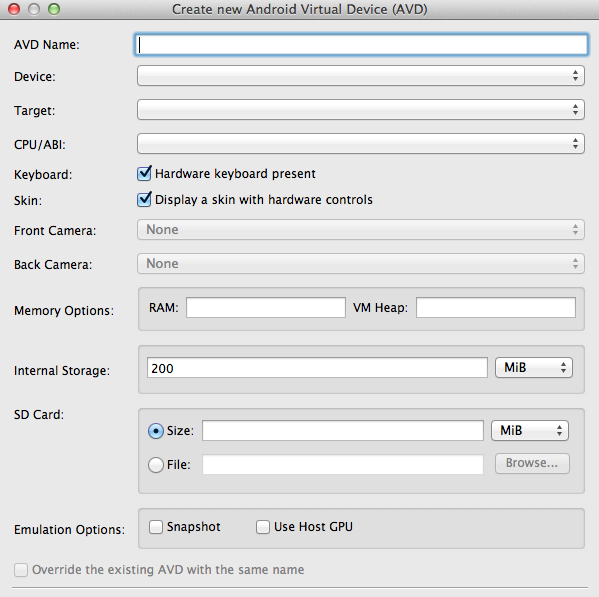
\includegraphics[scale=0.5]{figures/avd.png}
 \caption{Android Virtual Device configuration}
 \label{fig:avd}
\end{figure}

The Android emulator boots an Android image according to the \gls{avd} configuration file. The \gls{avd} allows to define hardware and software characteristics of a specific model to run on the Android emulator. \autoref{fig:avd} shows a snapshot of the \gls{avd} window configuration. For instance, in the \textit{Device} option it is possible to choose an Android model, as \textit{Nexus 4}, \textit{Nexus 7}, \textit{Nexus 10}, \textit{Galaxy Nexus}, \textit{Nexus S}, etc. The \textit{Target} element defines the Android version and the corresponding \gls{api}, as \textit{Android 2.3.3 - API Level 10}, \textit{Android 4.4 - API Level 19}, etc.

Once the \gls{avd} is created, the emulator may be launched through the \gls{avd} Manager or using the command line. Some useful commands\footnote{http://developer.android.com/tools/help/emulator.html} are presented as follow.

\begin{lstlisting}[caption=Command to start the Android emulator]
# emulator -avd <avd_name>
\end{lstlisting}

This command launches the emulator with the \gls{avd} image called \textt{avd\_name}. \gls{avd} files are usually stored at \texttt{.android/avd/} within the Android \gls{sdk} folder.

\begin{lstlisting}[caption=Command to provide a kernel to the Android emulator]
# emulator -avd <avd_name> -kernel <kernel_path>
\end{lstlisting}

In order to choose a kernel of our own, to run on the emulator, it is used the \texttt{-kernel} flag followed by the path of the image kernel file.

 \begin{lstlisting}[caption=Command to provide kernel prints of the Android emulator]
# emulator -avd <avd_name> -kernel <kernel_path> -show-kernel -verbose
\end{lstlisting}

To follow what is happening during the boot and to inspect kernel prints, the emulator provides both \texttt{-show-kernel} and \texttt{-verbose} flags.

\subsection{Android Debug Bridge}

\gls{adb}\footnote{http://developer.android.com/tools/help/adb.html} is another useful tool that connects the computer to Android devices (real or emulated). This connection brings powerful features that will be described in this section. The \gls{adb} tool, mention as adb from now on, is available as a command line. It is a client-server program that comprises three components:

\begin{itemize}
\item A client, that runs on the development computer;
\item A server, that runs as a background process on the development computer. The server handles communication between the client and the daemon;
\item A daemon, that runs in background on the mobile device (real or emulated).
\end{itemize}

Once Android emulator is started, adb provides a means of communication. The following command shows all Android devices running on the computer:

 \begin{lstlisting}[caption=Command to show Android devices running on the computer]
# adb devices
\end{lstlisting}

If there is an Android emulator running on the computer, the output returned is similar to the following:

 \begin{lstlisting}[caption=Example of the output from the \texttt{adb devices} command]
List of devices attached 
emulator-5554	device
\end{lstlisting}

With adb it is possible to:

\begin{itemize}

\item install an Android application on the emulator/device;
 \begin{lstlisting}[caption=Command to install Android apps using the adb utility]
# adb install <path_to_apk>
\end{lstlisting}

\item copy a specific file from the emulator/device to the development computer;
 \begin{lstlisting}[caption=Command to pull files using the adb utility]
# adb pull <remote> <local>
\end{lstlisting}

\item copy a specific file from the development computer to the emulator/device;
 \begin{lstlisting}[caption=Command to push files using the adb utility]
# adb push <local> <remote>
\end{lstlisting}

\item print the logcat output;
 \begin{lstlisting}[caption=Command to get logcat's prints using the adb utility]
# adb logcat
\end{lstlisting}

\item start a remote shell in the target emulator/device:
 \begin{lstlisting}[caption=Command to start a remote shell using the adb utility]
# adb shell
\end{lstlisting}

\end{itemize}

There are more options to execute with adb that can be checked on the Android online page\footnote{http://developer.android.com/tools/help/adb.html}.

\section{Android NDK and JNI}
Android provides a powerful toolset that has multiple purposes, available at \url{http://developer.android.com/tools/sdk/ndk/index.html}.  The Android \gls{ndk} was built to supply developers the capability to exploit the full power of mobile devices using native code. This is achieved through the \gls{jni}, which is a programming framework that provides connection between Java code that runs on the virtual machine and native code, as C/C++. Native code is accessed by the Java side as a static library, declared through the following statement:

\begin{lstlisting}[style=JavaInputStyle]
static { 
  System.loadLibrary("native");
}
\end{lstlisting}

This \texttt{native} library implements a set of native methods called in Java. For instance:

\begin{lstlisting}[style=JavaInputStyle]
public native void nativeMethodA();
public native String nativeMethodB(String str);
\end{lstlisting}

At this point, Java knows that in order to execute the \texttt{nativeMethodA()} and the \texttt{nativeMethodB()}  it has to inspect the \texttt{native} library stored as \texttt{libnative.so} placed at \texttt{libs/armeabi/} in the Android project folder.

This library consists of, at least, three files that should be placed at a folder called \texttt{jni}:

\begin{itemize}
\item the \texttt{Android.mk} configuration file;
\item the header file;
\item the C/C++ file.
\end{itemize}

The \texttt{Android.mk} file comprises several configurations required by the \textit{ndk-build} tool. This tool is brought by the Android \gls{ndk} and allows to compile native code generating library files as well as executable files. The minimum intructions of an \texttt{Android.mk} file are presented as follows:

\begin{lstlisting}[style=CInputStyle]
LOCAL_PATH := $(call my-dir)
 
include $(CLEAR_VARS)
       
LOCAL_MODULE    := native
LOCAL_SRC_FILES := native.c

include $(BUILD_SHARED_LIBRARY)
\end{lstlisting}

This file specifies the native source files location, in \texttt{LOCAL\_PATH}, the name of both the library and the native code file, in \texttt{LOCAL\_MODULE} and \texttt{LOCAL\_SRC\_FILES}. The statement \texttt{CLEAR\_VARS} indicates no dependent configuration disrupts compilation \cite{AndroidNDK:Packt}. At last \texttt{BUILD\_SHARED\_LIBRARY} instructs to build a shared library.

The header file name follows a pattern: \texttt{<package\_name>\_<class>.h} . Imagine that the Java class that loaded the library is called \texttt{LoadLibrary} and the Java package that contains this class is called \texttt{com.android.droidguardian}. The name of the header file will be: \\
\texttt{com\_android\_droidguardian\_LoadLibrary.h}\\
\noindent This file is automatically generated by a tool called \textit{javah} provided by the \gls{jdk}. It was designed to build header files to the \gls{jni} and may be called as follows:

\begin{lstlisting}[style=BashInputStyle]
# javah -jni -d <path_to_jni_folder> -classpath <path_to_class_files> com.android.droidguardian.LoadLibrary
\end{lstlisting}

This tool operates over \texttt{.class} files which means that the Java code must be compiled before.

The native code goes on regular \texttt{.c/.cpp} files. The next section will introduce basic \gls{jni} concepts in order to get a native library running on Java.

\subsection{JNI concepts}




\section{Android development}
The Android OS was designed to achieve the best performance when running in mobile devices. This goal brings particular characteristics that developers need to bear in mind when creating Android apps. Some of these characteristics are introduced in this section.

\subsection{Application Not Responding}

Android is built to be highly responsive, which means components may not block on I/O operations on the main thread (also known as the \gls{ui} thread). The system must always be available to respond to user input events. Whenever an application is using the main thread, Android triggers an internal clock that fires when one of the following conditions occurred:

\begin{itemize}
\item No response to an input event within 5 seconds.
\item A BroadcastReceiver hasn't finished executed within 10 seconds.
\end{itemize}

Then, the system launches an \gls{anr} dialog window allowing the user to stop the application's execution, as illustrated in \autoref{fig:anr_dialog}.

\begin{figure}[h]
 \centering
 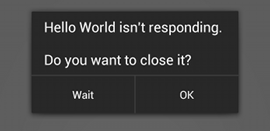
\includegraphics[scale=0.5]{figures/anr_dialog.png}
 \caption{Application Not Responding dialog window}
 \label{fig:anr_dialog}
\end{figure}

To avoid \gls{anr} dialogs, it is recommended to use worker threads in order to execute heavy and long tasks that would block the main thread. The following section introduces the use of worker threads on Android.

\subsection{Worker Threads}

Android consists of four main components that were presented earlier: Activities, Services, Broadcast Receivers and Content Providers. When an application starts executing, Android initiates a new process and, usually, all components run in the same process and thread (main thread). This thread is also called the \gls{ui} thread, because it supports the Android \gls{ui} toolkit components (from the \texttt{android.widget} and \texttt{android.view} packages) that applications interact with. When users provide \gls{ui} events, such as touching a button on the screen, the event is enqueued until the \gls{ui} thread is ready to dispatch it. If some application's component starts a heavy task, by default, it will run on the \gls{ui} thread which may lead to a blocking situation where user input events get stuck on the queue \cite{ProAndroid4:Apress}. This is the typical case where \gls{anr} dialogs are prompted.

Worker threads are used to overcome this problem. In order to take off heavy tasks from the \gls{ui} thread so that it can be ready to handle \gls{ui} events, developers must create other threads to execute such tasks. Note that \gls{ui} events cannot be handled by worker threads, which means that developers may not access the Android \gls{ui} toolkit outside the main thread.


\chapter{Implementing Droidguardian}
\label{chap:implementing_dg}



\section{Setting up the environment}

The development process of DroidGuardian comprised several stages that corresponding to the layer level that was being handled. The kernel module requested a completely different environment when compared to the Java layer implementation environment.

In order to fully understand the \gls{lsm} framework it was necessary to manipulate a real Linux kernel, as well as compile and install. Since the work machine used was a \textit{MacBook Pro}, a new partition was created to install the \textit{Xubuntu}. This is a different flavor of \textit{Ubuntu Linux} operating system that provides a light user interface. Basically, the only used program was the console, because all required steps could be executed through the command line and using \textit{Vim}. This is why a lighter and simpler user interface was enough to carry on the desired tasks on the Linux environment. The new partition was created using \textit{rEFIt}\footnote{http://refit.sourceforge.net}.

Running Linux on a new partition provided speed and efficiency when setting up the Android environment, to build and launch a new image on the emulator. However, handling loadable kernel modules on a separated partition proved to be a mistake, due to the system's blocking when kernel failures were reached by programming errors. To overcome this inconvenience, programming tests with loadable kernel modules started to be done in a virtual machine. This way, if the code contained flaws that could led to a kernel panic, the virtual machine could easily be restarted causing no pain to the host operating system. \textit{VMWare} was used to virtualize a \textit{Xubuntu} operating system, being \textit{OS X} the host operating system.

Regarding the Android application development environment, \textit{Eclipse} was chosen as the \gls{ide}, because is widely used, well documented and almost all issues an user may face are solved in internet forums, books and other sources.

Application testing was conducted on both the Android emulator and a real device. The device was a \textit{Commtiva z71} running Android 2.3.3, \gls{api} level 10.

\section{Kernel Module}

The main challenge in this project consisted in the manipulation of hook functions to properly handle socket connections at kernel level.

\section{Native layer}

Users control internet connection attempts through an Android application. This application may be divided into two layers: \textit{Native layer} and \textit{Java layer}. This section introduces the former and the following section presents the last.


\section{Java layer}

The topmost layer of DroidGuardian has the only purpose of displaying the data to the user. This is achieved through an Android application, that is provided with both the necessary components and a powerful \gls{api}. Android components, presented in a previous chapter, were carefully studied in order to ensure that DroidGuardian was being built with the proper pieces. However, when compared to the usual Android applications lifecycle, DroidGuardian may be seen as a different kind of application that was not though to follow the good tips when it concerns the behavior of applications in mobile environments. But, more on that later.

\begin{figure}[h]
 \centering
 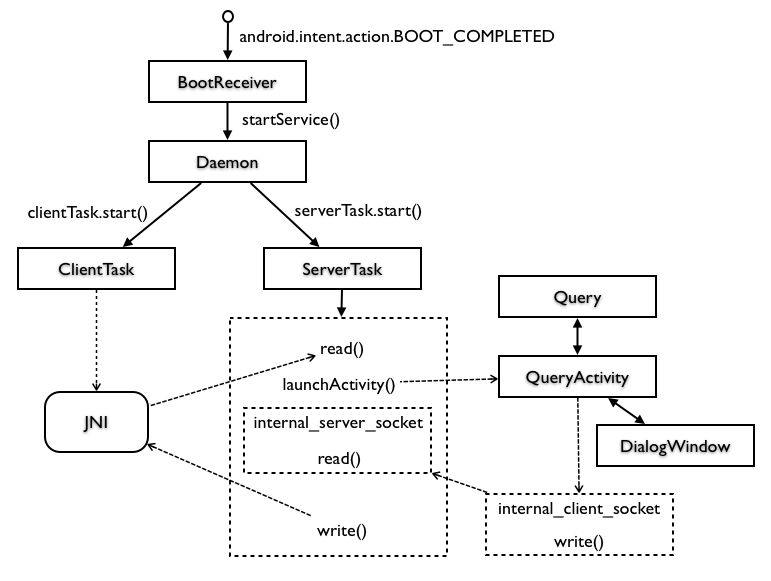
\includegraphics[scale=0.5]{figures/dg_java_flow.png}
 \caption{Process flow in the Java layer}
 \label{fig:dg_java_flow}
\end{figure}

The process flow of the Java layer is illustrated in \autoref{fig:dg_java_flow}. It presents the following classes:

\begin{itemize}
\item \texttt{BootReceiver}: operates as a \textit{BroadcastReceiver} that starts DroidGuardian after the device booting process.
\item \texttt{Daemon}: acts as a \textit{Service} to run in background while the device is on.
\item \texttt{QueryActivity}: is the \textit{Activity} responsible for displaying the data of queries to the user.
\item \texttt{Query}: does not extend an Android component, being used to translate a native query into a Java query.
\item \texttt{DialogWindow}: is bounded to the \texttt{QueryActivity}, building a fragment to display the dialog window.
\end{itemize}

DroidGuardian was design to run as a daemon, silently and unnoticed, until internet connection requests arose to trigger the dialog window.  Also, applications may launch internet requests at any time since the device starts running. Therefore, DroidGuardian needs to start listening as soon as possible. Android fires an intent immediately after the booting process, allowing applications to receive it:

\indent \texttt{android.intent.action.BOOT\_COMPLETED}

This intent is received trough \textit{Receivers} or \textit{BroadcastReceivers} that overwrite a callback named \texttt{onReceive()}. This method is responsible for grabbing intents and triggering whatever action the developer wants. In this case, the \texttt{BootReceiver}'s \texttt{onReceive()} method starts the daemon allowing DroidGuardian to connect to the kernel module and start listening internet requests.

The following steps describe the process flow of the Java layer:

\begin{enumerate}
\item Android sends \texttt{BOOT\_COMPLETED} intent action and \texttt{BootReceiver} grabs it.
\item \texttt{BootReceiver} starts the service \texttt{Daemon} after grabbing the intent.
\item The \texttt{Daemon} service launches two threads: \texttt{ServerTask} and \texttt{ClientTask}. The former operates as a server in the stream socket protocol and will run until an external perturbation, as low memory, destroys the service. If nothing happen, this socket server will run while the device is on. The last acts as the client socket in this connection. However, the client code is not implemented in this class but in the native library. This thread calls the native method \texttt{startDaemon()} that kicks off the native engine.
\item Once executing, the server socket starts a \texttt{while(1)} loop in which queries' data will be exchanged between the server and the client.
\item When the client gets a query sends it to the server, that receives it through the \etxttt{read()} method of the \texttt{InputStream} interface.
\item Immediately after reading the query, the server invokes an instance of the \texttt{QueryActivity} class through intents, transmitting the query's data.
\item Along with this call to \texttt{QueryActivity}, the server also initializes a new server socket, called internal server, that will handle the communication between the \texttt{Daemon} and the \texttt{QueryActivity}.
\item The \texttt{QueryActivity} gets the query's data in a special format. Then, creates an instance of the \texttt{Query} class, which has as instance variables the fields that will ultimately display the information to the user.
\item This process culminates with the execution of the \texttt{DialogWindow}. The \texttt{QueryActivity} instantiates a new Activity Fragment and exhibits it through the \texttt{show()} method.
\item The \texttt{DialogWindow} fills itself with a View that contains a text, a spinner and buttons. The text displays the internet connection request information so that the user may decide what option to chose in the spinner and what button to click on.
\item Once the user clicks a button, the \texttt{DialogWindow} executes a method that provides from a Java Interface and is implemented in the \texttt{QueryActivity} class. This method starts the internal client socket that will send the user's action to the internal server, listening on the \texttt{Daemon}'s server loop. After sending the message, the internal client closes itself.
\item The internal server gets the information, stores it in a variable and closes itself.
\item At last, the server reads this variable's value and sends the message back to the native client.
\item This process is repeated every time a new connection request reaches the Java layer.
\end{enumerate} 

\section{Decisions}

While developing DroidGuardian, various doubts and questions came out regarding the best way to implement certain features. This section presents those cases along with the decision taken and its explanation.

\subsubsection{Dialog vs Notification}

The dialog window don't follow the correct rules that Android states when it comes to alert the user that some event occurred. Dialogs exist for this purpose, but in a different context. A dialog alert should be used inside an activity that the user intentionally invoked. For instance, when the user triggers an action to delete data from a certain folder it is expected that a dialog window pops up asking if he intends to delete that data. This is a consequence of the user's action.

In situations where an event occurs outside the application that the user is interacting with, Android offers the \textit{Notification} interface. Notifications are messages displayed on the notification bar, placed at the top (or bottom) of Android devices, by icons. When a new icon appears on the notification bar, it means that some event took place as a result from a background action. The user is able to expand the notification bar to check all notifications that, usually, comprise some short information text. By clicking on the notification area, it may fill the screen with data related to the event that occurred, depending on how the notification was developed. Users are free to keep notifications unread for as long as they want, without lose performance.

Considering both elements, dialogs and notification, the DroidGuardian case fits better in the last, because the event that triggers an alert to the user happens in background. However, taking the internet connection request to the notification bar would lead to a longest response time when compared to the dialog. The time the user takes to provide his input is included in the total amount of time that the socket waits in the kernel in order to accept or reject the connection. It is known that kernel operations should be executed as fast as possible and that keeping the kernel stuck could bring several damages to the system. Even though it is kept waiting a considerable amount of time using dialogs, compared to notifications this time would increase. 

It was decided that disrupt the user from whatever he is doing, with an alert pop up was better than keeping the kernel waiting long periods of time.

\subsubsection{Service and Activity communication}

The communication between the \texttt{Daemon} and the \texttt{QueryActivity} is established through local sockets. This is the third nested socket connection that takes place since DroidGuardian intercepts an internet connection attempt in the kernel and displays it to the user.



\chapter{Using Droidguardian}
\label{chap:using_dg}
\input{using_dg}

\chapter{Conclusion}
\label{chap:conclusion}
Conclusion and Future Work

%%%%% END OF THESIS CONTENT %%%%%%%
\renewcommand{\bibname}{References}
\bibliographystyle{ieeetr}
\bibliography{bibliography.bib}
\addcontentsline{toc}{chapter}{References}

%\appendix
%\chapter{User manual in Portuguese}\label{appManual}
%\thispagestyle{empty} \cleardoublepage
%\includepdf[pages=5-68, nup=1x1, frame=true, link=true, linkname=anexomanual]{ManualUtilizador.pdf} 
    

\end{document}
